%%%%%%%%%%%%%%%%%%%%%%%%%%%%%%%%%%%%%%%%%%%%%%%%%%%%%%%%%%%%%%%%%%%%%%%%%%%%%%%%
%% 实验报告模板.tex                                                           %%
%% author: hxp<hxp201406@gmail.com>                                           %%
%% 按照基础物理实验老师发的模板更改形成                                       %%
%%%%%%%%%%%%%%%%%%%%%%%%%%%%%%%%%%%%%%%%%%%%%%%%%%%%%%%%%%%%%%%%%%%%%%%%%%%%%%%%
%% 备注:刚刚的注释刚好是80行,编写代码的时候不要超过80行,就是你的代码不要超 %%
%% 过我注释里面最后面的“%”,超过请换行。                                      %%
%%%%%%%%%%%%%%%%%%%%%%%%%%%%%%%%%%%%%%%%%%%%%%%%%%%%%%%%%%%%%%%%%%%%%%%%%%%%%%%%
%% 模板现在开始,请根据注释把相应的位置更改成对应的内容                       %%
%%%%%%%%%%%%%%%%%%%%%%%%%%%%%%%%%%%%%%%%%%%%%%%%%%%%%%%%%%%%%%%%%%%%%%%%%%%%%%%%


\documentclass{ctexart}


\usepackage{ctex}
\usepackage{amsmath}
\usepackage{amsfonts}
\usepackage{amssymb}
\usepackage{wasysym}
\newcommand{\angstrom}{\text{\normalfont\AA}}  % 定义了原子物理的A
\usepackage{graphicx}
\usepackage{float}
\usepackage{geometry}
\geometry{a4paper,scale=0.8}  % 定义页面大小是A4,缩放是0.8
\usepackage{caption}
\usepackage{subcaption}
\usepackage{enumitem}

\newcommand*{\md}{\mathop{}\!\mathrm{d}}   % 定义微分算子,直立体的d
\newcommand*{\me}{\mathrm{e}}              % 定义自然对数e,同样应当是直立体

% 如果你想要每一段的开头不要空两格,注释掉下面这两行
% \usepackage{parskip}
% \setlength{\parindent}{0cm}

% 默认的\mathbf对希腊字母不生效,这里改下
\usepackage{bm}
\let\Oldmathbf\mathbf
\renewcommand{\mathbf}[1]{\boldsymbol{\Oldmathbf{#1}}}

% 表格默认格内内容和边框没有留出距离,显示分数的时候,分数的上下会贴到边框上
% 因此我增加了表格内容和边框的最短距离是5像素
\usepackage{cellspace}
\setlength{\cellspacetoplimit}{5pt}
\setlength{\cellspacebottomlimit}{5pt}

% \si命令是用来写单位的,单位需要和之前的数字有一个空格的距离,而且应当直立体
% 用法:5 \si{km/h}
\newcommand{\si}[1]{\  \mathrm{#1}}

% 日期不要显示
\date{}

\usepackage{fancyhdr}
\pagestyle{fancy}
\fancyhf{}
\lhead{本文档TeX源码地址:https://github.com/hxp-plus/Notes/tree/master/Physics-Experiment/实验报告}
\rfoot{第 \thepage 页}
\renewcommand{\headrulewidth}{1pt}
\renewcommand{\footrulewidth}{1pt}

%% 标题三号黑体,作者信息为班级姓名学号
\newcommand{\generatetitle}[6]{\title{\zihao{3}\heiti#1} \author{#2 \quad
    \quad #3 \quad\quad #4 \quad\quad #5 \quad\quad #6} \maketitle\thispagestyle{fancy}}

%% 所有的引言、实验内容与数据处理啥的,用section
\ctexset {
  section = {
    format = \raggedright\zihao{4}\heiti,  % 设置所有section的字号为四号黑体左对齐
    name={,、},                            % 序号后跟顿号
    aftername={\hspace{0pt}},              % 修改序号和标题直接的间距为零
    number=\chinese{section},              % 设置序号为中文
  },
  subsection = {
    format = \raggedright\zihao{5}\heiti,  % 设置所有subsection的字号为五号黑体左对齐
    number={},              % 设置序号为没有序号
  }
}

%% 实验背景、实验目的啥的,用subsection
\ctexset {
  subsection = {
    format = \raggedright\zihao{5}\heiti,  % 所有subsection的字号为五号黑体左对齐
    number={},                             % 设置序号为没有序号
  }
}

%% 把subsection之间加上中括号
\let\oldsubsection\subsection
\renewcommand{\subsection}[1]{\oldsubsection{\!\!\!\!\!\!【#1】}}

%% 摘要和关键词用paragraph

\ctexset {
  paragraph = {
    format = \raggedright\zihao{5}\heiti,  % 所有paragraph的字号为五号黑体左对齐
    number={},                             % 设置序号为没有序号
  }
}

%% 把paragraph之间加上中括号
\let\oldparagraph\paragraph
\renewcommand{\paragraph}[1]{\oldparagraph{#1:\!\!\!\!\!\!}}

%% 再把参考文献的序号去掉
\makeatletter
\renewcommand\@biblabel[1]{}
\makeatother

\begin{document}

\generatetitle{近代物理实验报告——
  双频外差激光干涉仪}{物理4+4}{胡喜平}{U201811966}{hxp201406@gmail.com}{https://hxp.plus/}

\paragraph{摘要}
光的干涉在精细的测量中有广泛的应用,双频外差激光干涉仪就是一例。本次实验搭建双频外差激光干涉仪,来探索它的性质。

% 关键词
\paragraph{关键词}
双频外差激光干涉、声光调制器

\section{引言}

\subsection{实验目的}
掌握声光调制器的使用方法,搭建双频外差激光干涉仪光路,观察参考光和测量光的信号。

\section{实验内容与数据处理}
\subsection{实验原理}

\textbf{非偏振双频激光干涉仪}如图所示,其中两束氦氖激光存在无论是到PD1还是PD2都存在一定的光程差,为了方便讨论将图上四个位置用字母A、B、C、D表示。PD表示光电测量器,AOM表示声光调制器。

\begin{figure}[H]
  \centering
  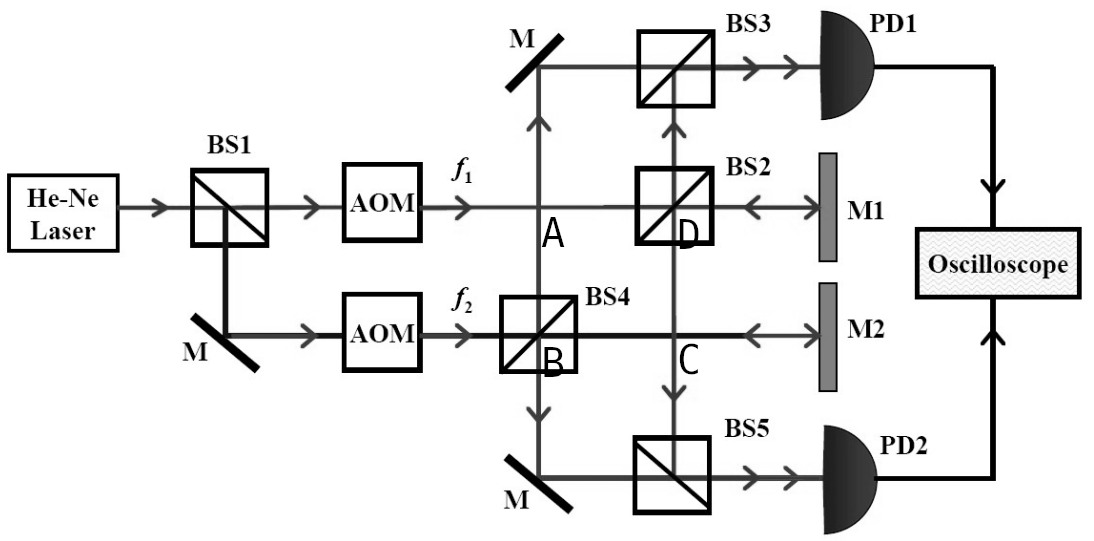
\includegraphics[width=0.9\linewidth]{figures/非偏振双频激光干涉仪}
  \caption{非偏振双频激光干涉仪示意图}
\end{figure}

其中抵达PD1的是参考光,抵达PD2的是测量光。实验中直接测量的量是两组干涉激光的测量信号的相位差$\Delta \phi$,间接测量反射镜M2与M1的相对位移$\Delta L$。

我们假设刚开始两个反射镜水平方向是没有位移的,那么对于\textbf{参考光},频率为$f_2$的光比频率为$f_1$的光多走的距离是$2 \overline{AB}$。而对于\textbf{测量光},频率为$f_2$的光比频率为$f_1$的光多走的距离是$2 \overline{BC}$。

因此为了防止出现奇怪的情况,在搭建实验光路的时候,应当尽量让这个系统保持是二维的,不要让光有竖直方向的偏差。其中实验中测量到的信号的光强信号为:

\begin{itemize}
\item 参考光:$I_r \propto I_0 \cos \left[ 2 \pi \left( f_1 - f_2 \right)t + \left( \varphi_{01} - \varphi_{02} \right) \right] $
\item 测量光:$I_m \propto I_0 \cos \left[ 2 \pi \left( f_1 - f_2 \right)t + \left( \varphi_{01} - \varphi_{02} \right) + \Delta \phi \right] $
\end{itemize}

两个反射镜之间的相对位移为:

\begin{equation*}
  \begin{aligned}
    \Delta L = \dfrac{\lambda}{4 \pi} \Delta \phi 
  \end{aligned}
\end{equation*}

下面是一个\textbf{偏振双频激光干涉仪}示例

\begin{figure}[H]
  \centering
  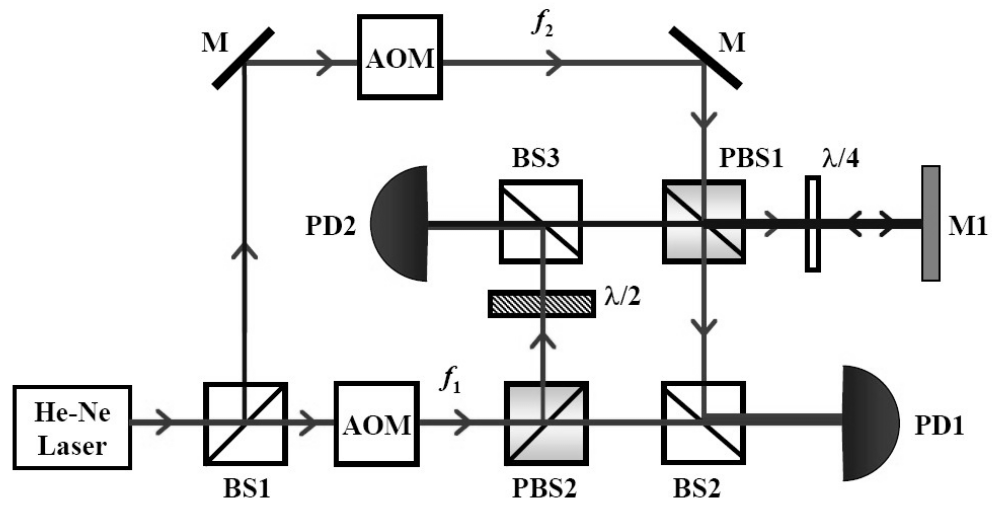
\includegraphics[width=0.9\linewidth]{figures/偏振双频激光干涉仪}
  \caption{偏振双频激光干涉仪示意图}
\end{figure}

通过移动反射镜M1,造成测量光的相位发生变化,由于M1到PBS1的距离光走一来一回了两遍,反射镜位移和相位差之间的关系依然是:

\begin{equation*}
  \begin{aligned}
    \Delta L = \dfrac{\lambda}{4 \pi} \Delta \phi
  \end{aligned}
\end{equation*}

因此用示波器测量$\Delta \phi$可以间接测量$\Delta L$。

\subsection{实验内容}

\begin{itemize}
\item 使用声光调制器对激光光束进行调制,产生不同频率的激光。搭建\textbf{非偏振双频外差激光干涉仪}光路。
\item \textbf{不考虑偏振}的情况下,观察和比较参考光和测量光的干涉信号,通过两干涉信号相位差测量决定光程差,得出\textbf{相位差}与\textbf{反射镜移动位移}的函数关系。
\item 考虑偏振的情况下,设计\textbf{基于偏振的双频外差激光干涉仪},重复上述测量。
\end{itemize}

\subsection{实验结果的分析和结论}

我们在实验中由于不知道光学实验的操作要领,光学实验经验不足,前期光路总是调不好,浪费了太多时间。最终还是搭建好了测量光和参考光的光路。实验中我们曾经4次搭好参考光路,得到的示波器图像如下

\begin{figure}[H]
  \centering
  \begin{subfigure}{.96\textwidth}
    \centering
    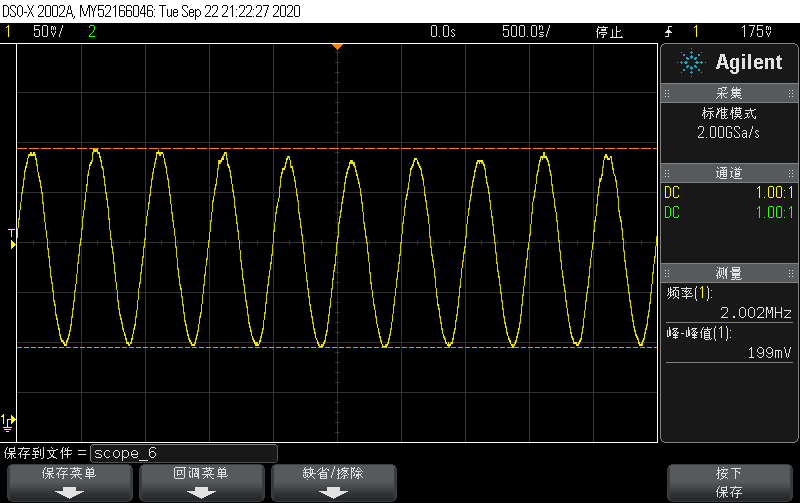
\includegraphics[width=\linewidth]{双频激光干涉装置图像/参考光4}
    \caption{实验中得到的最好的参考光图像,是最后一个出来的图像,那时候我们已经掌握了做光学实验的要领}
  \end{subfigure}
  \begin{subfigure}{.32\textwidth}
    \centering
    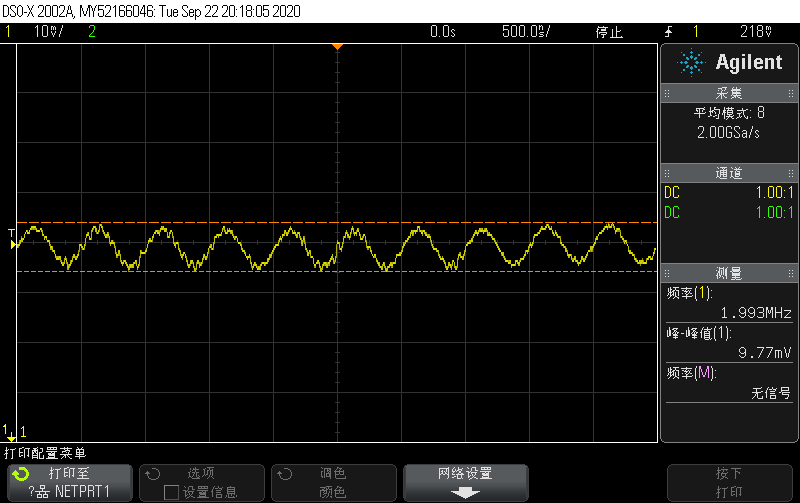
\includegraphics[width=\linewidth]{双频激光干涉装置图像/参考光1}
    \caption{第一次测量到参考光的图像}
  \end{subfigure}
  \begin{subfigure}{.32\textwidth}
    \centering
    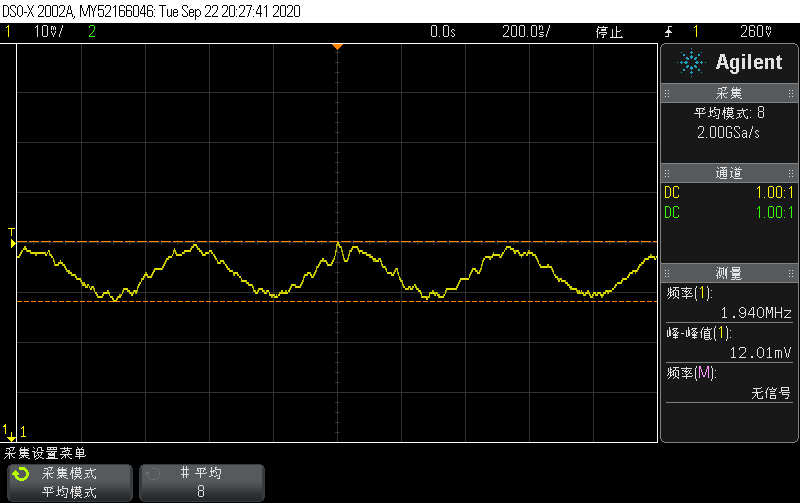
\includegraphics[width=\linewidth]{双频激光干涉装置图像/参考光2}
    \caption{第二次测量到参考光的图像}
  \end{subfigure}
  \begin{subfigure}{.32\textwidth}
    \centering
    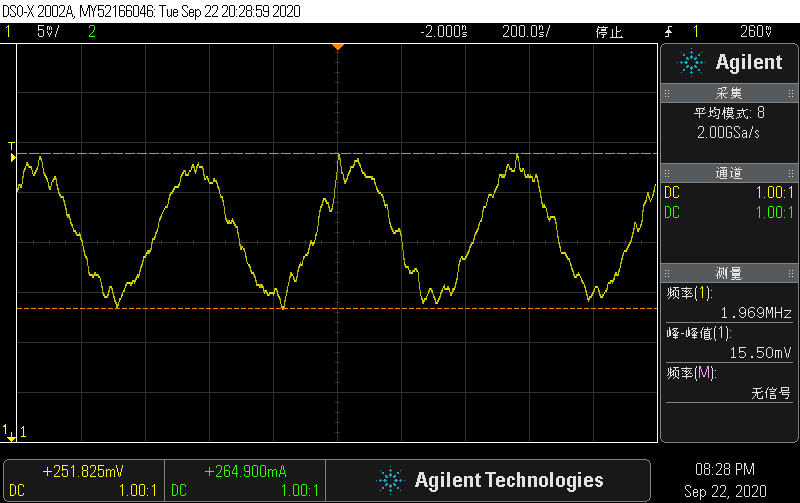
\includegraphics[width=\linewidth]{双频激光干涉装置图像/参考光3}
    \caption{第三次测量到参考光的图像}
  \end{subfigure}
  \caption{实验中得到的参考光图像}
\end{figure}

同时我们使用参考光的搭建经验来搭建了测量光。测量光由于经过了多次反射与透射,光的强度远没有参考光强,因此参考光的探测器有测量光10倍的灵敏度。我们反复对准光路,已经竭尽全力使得光路是保持在二维平面内对准的状态,但是依旧没有得到稳定的图像。后面我们尝试关掉实验室里的灯来使激光看起来更亮,因为测量光实在太弱了,肉眼不仔细看很难看见,关灯后能看的比较清楚,调节光路的时候会更精准。但是即使是这样还是只能在示波器里面得到模糊的图像,图像只能勉强看出是驻波,频率根本无法测量,因此也没有办法用来测量光的相位差。下面是我们得到的一些图像

\begin{figure}[H]
  \centering
  \begin{subfigure}{.48\textwidth}
    \centering
    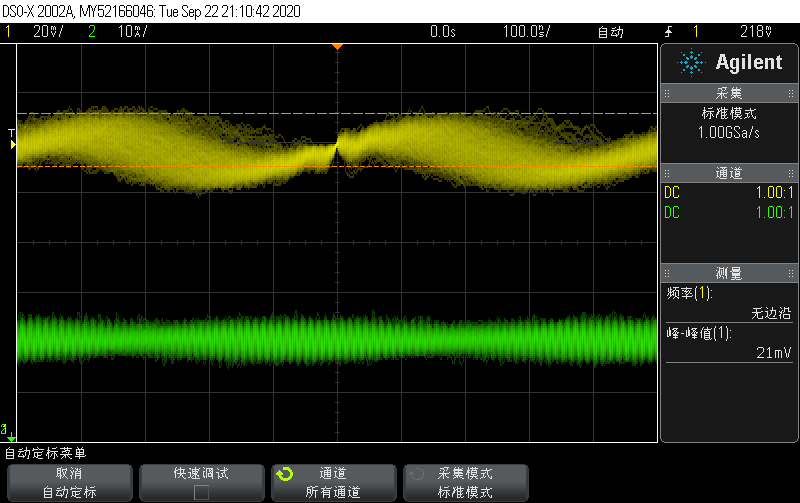
\includegraphics[width=\linewidth]{双频激光干涉装置图像/测量光和参考光1}
  \end{subfigure}
  \begin{subfigure}{.48\textwidth}
    \centering
    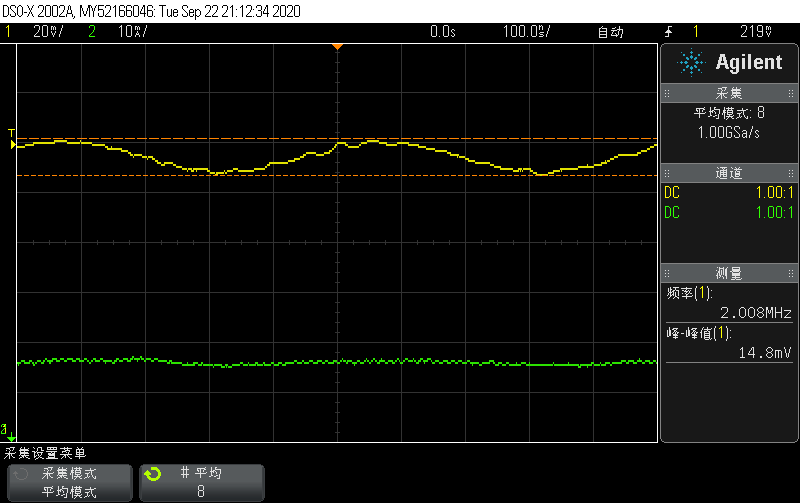
\includegraphics[width=\linewidth]{双频激光干涉装置图像/测量光和参考光2}
  \end{subfigure}
  \caption{实验中得到的测量光图像}
\end{figure}

图像里参考光一点问题都没有,频率也测出来是2MHz,但是测量光就是测不出频率。可能是激光光源不够强,也可能是环境噪声太大或者是仪器不够好。

\subsection{实验中遇到的问题及解决方法}

通过这次光学实验我找到了光学实验的要领,就是每一步都要保持光在同一平面。是否光还是平行于实验台需要拿尺子测量,在近处测量一次光到实验台的距离,远处测量一次,距离不能有肉眼可见的一点偏差。

\section{参考文献}
\begin{itemize}[leftmargin=0pt]
  \item[] 近代物理实验讲义
\end{itemize}
\end{document} 
